%!TEX root = ../thesis.tex
% \chapter*{付録}
\appendix
\renewcommand{\thesection}{A.\arabic{section}}
% \renewcommand{\thetable}{A.}
\renewcommand{\thefigure}{A.\arabic{figure}}
\chapter{付録A}
\label{chap:appendix}
% \addcontentsline{toc}{chapter}{付録}
\vspace{-18pt}
\section{動画}
\ref{chap:application}章のシステムを用いて,シミュレータ環境で歩行者の将来位置の予測結果を可視化している様子を動画に記録した.以下に動画のURLを掲載する.
\\
\url{https://youtu.be/-49zaStfWhs}

\section{ロボットと歩行者の軌道と時間変化の可視化例}
\figref{Fig:cross-viz}と\figref{Fig:block-viz}に,\ref{chap:experiments_pred_sim}章の実験におけるシナリオ1およびシナリオ2でのロボットと歩行者の位置の時間変化の一例を示す.
 
\begin{flushleft}
  \textbf{シナリオ1}
\end{flushleft}

\figref{Fig:cross-normal}は,歩行者の位置予測結果を利用していないナビゲーションでの可視化例である.この例では,ロボットが歩行者の進行方向を妨げるように直進しており,歩行者が回避行動を取り,ロボットが先に進んでから歩行を再開していることが確認できる.

\figref{Fig:cross-pred}は,歩行者の位置予測結果を利用したナビゲーションでの可視化例である.この例では,ロボットが早期に停止し,歩行者が通り過ぎた後に走行を再開していることが確認できる.

\begin{flushleft}
  \textbf{シナリオ2}
\end{flushleft}

\figref{Fig:block-normal}は,歩行者の位置予測結果を利用していないナビゲーションでの可視化例であり,歩行者がロボットとすれ違う際に,回避行動を取っていることが確認できる.

\figref{Fig:block-pred}は,歩行者の位置予測結果を利用したナビゲーションでの可視化例である.この例では,ロボットが歩行者の進行方向を避けるように走行していることが確認できる.

\begin{figure}[H]
  \centering
  \begin{subfigure}{0.8\textwidth}
    \centering
    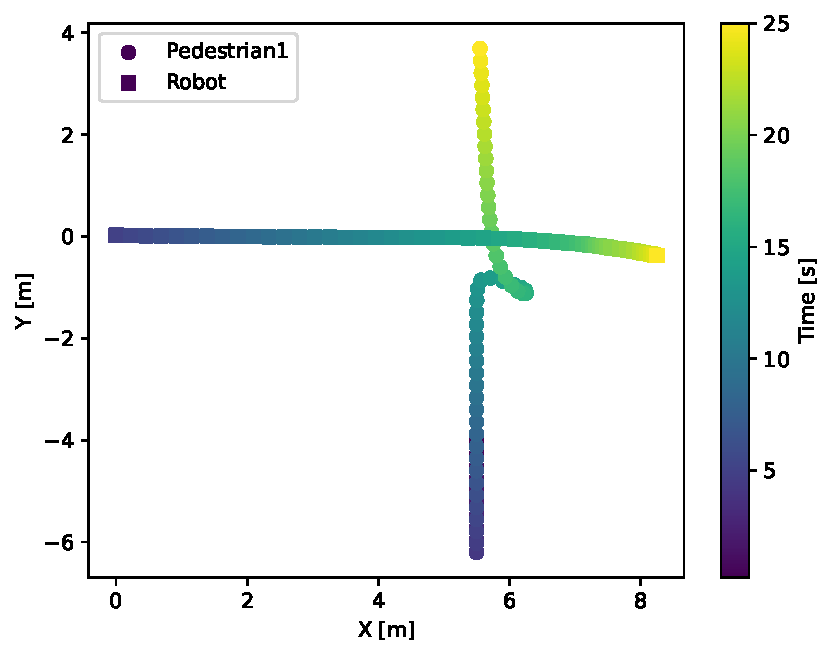
\includegraphics[keepaspectratio, scale=0.75]{images/cross_normal3.pdf}
    \caption{Navigation without prediction results}
    \label{Fig:cross-normal}
  \end{subfigure}
  \vfill
  \begin{subfigure}{0.8\textwidth}
    \centering
    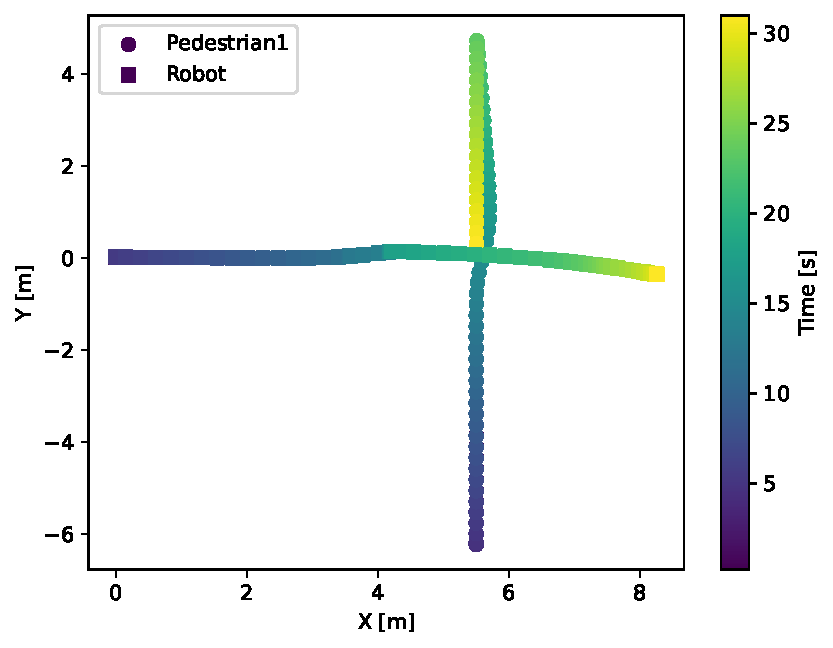
\includegraphics[keepaspectratio, scale=0.75]{images/cross_pred.pdf}
    \caption{Navigation with prediction results}
    \label{Fig:cross-pred}
  \end{subfigure}
  \caption{Position changes of the robot and pedestrian in scenario 1}
  \label{Fig:cross-viz}
\end{figure}

\begin{figure}[H]
  \centering
  \begin{subfigure}{0.8\textwidth}
    \centering
    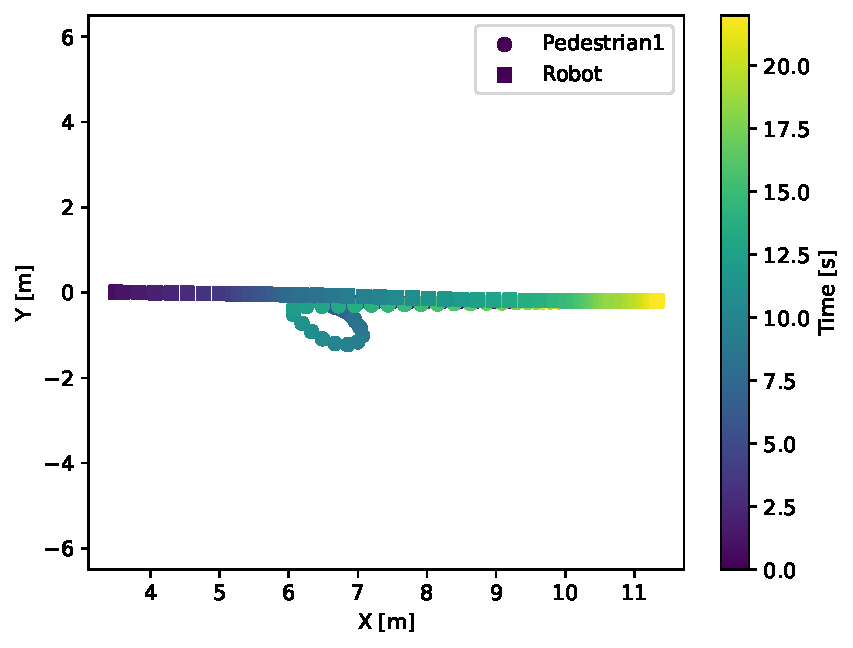
\includegraphics[keepaspectratio, scale=0.75]{images/block_normal.pdf}
    \caption{Navigation without prediction results}
    \label{Fig:block-normal}
  \end{subfigure}
  \vfill
  \begin{subfigure}{0.8\textwidth}
    \centering
    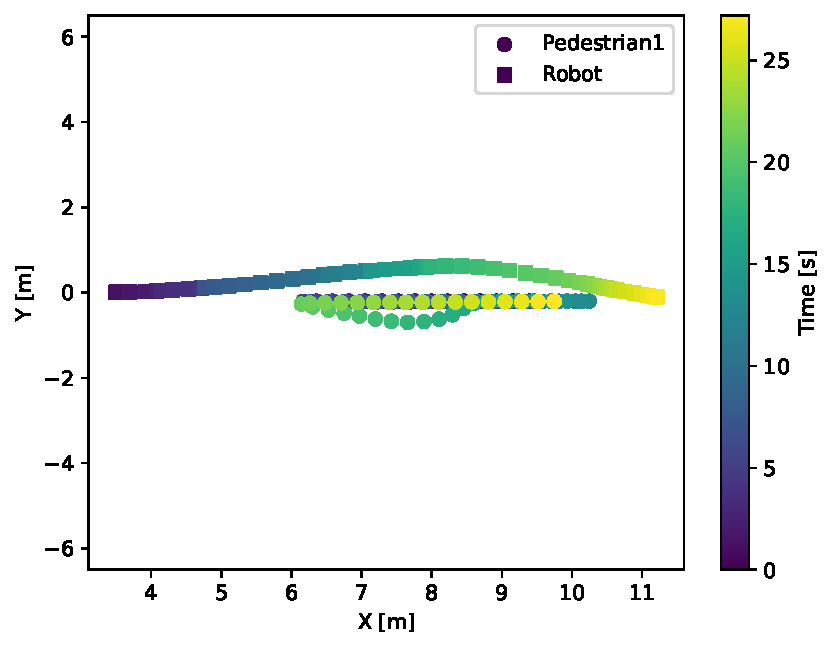
\includegraphics[keepaspectratio, scale=0.75]{images/block_pred.pdf}
    \caption{Navigation with prediction results}
    \label{Fig:block-pred}
  \end{subfigure}
  \caption{Position changes of the robot and pedestrian in scenario 2}
  \label{Fig:block-viz}
\end{figure}